%% Architecture Diagram — NEVEN Paper
%% Compile standalone: pdflatex architecture_diagram.tex
%% Or include via \input{} in main document

\documentclass[border=10pt]{standalone}
\usepackage{tikz}
\usetikzlibrary{shapes.geometric, arrows.meta, positioning, fit, backgrounds, calc}

\definecolor{excelgreen}{RGB}{00,00,00}
\definecolor{nevenblue}{RGB}{00,00,00}
\definecolor{rcolor}{RGB}{00,00,00}
\definecolor{juliacolor}{RGB}{00,00,00}
\definecolor{pythoncolor}{RGB}{00,00,00}
\definecolor{webviewcolor}{RGB}{00,00,00}
\definecolor{pipecolor}{RGB}{0,0,0}

%\definecolor{excelgreen}{RGB}{33,115,70}
%\definecolor{nevenblue}{RGB}{41,98,168}
%\definecolor{rcolor}{RGB}{39,109,195}
%\definecolor{juliacolor}{RGB}{149,88,178}
%\definecolor{pythoncolor}{RGB}{255,212,59}
%\definecolor{webviewcolor}{RGB}{0,120,212}
%\definecolor{pipecolor}{RGB}{180,180,180}

\begin{document}
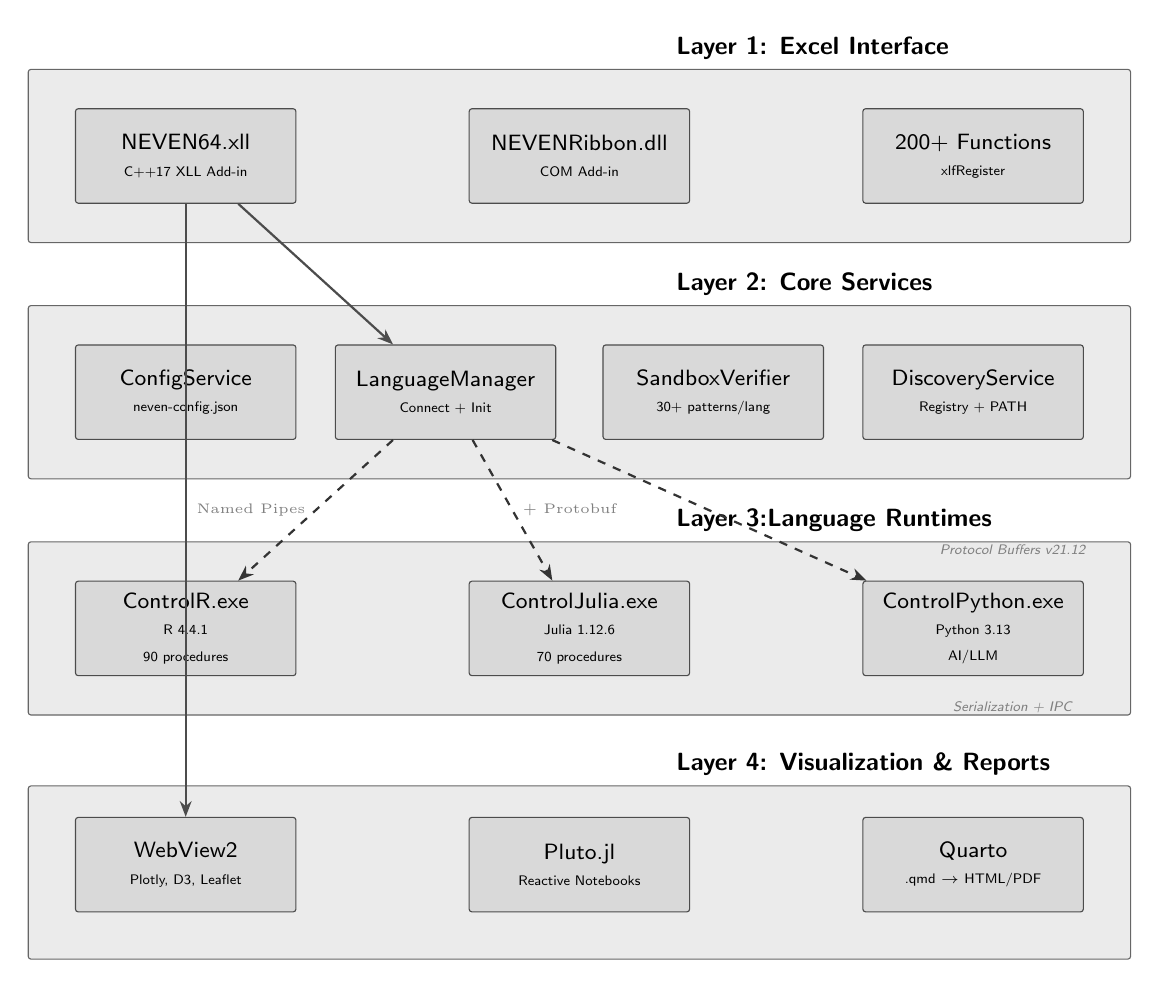
\begin{tikzpicture}[
    node distance=1.2cm and 2cm,
    every node/.style={font=\sffamily\small},
    layer/.style={draw, rounded corners=1pt, minimum width=14cm, minimum height=2.2cm, fill=#1!8, draw=#1!60},
    component/.style={draw, rounded corners=1pt, minimum width=2.8cm, minimum height=1.2cm, fill=#1!15, draw=#1!70, align=center, font=\sffamily\footnotesize},
    pipe/.style={-{Stealth[length=2mm]}, thick, draw=pipecolor!80, dashed},
    solidarrow/.style={-{Stealth[length=2mm]}, thick, draw=#1!70},
]

%% Layer 1: Excel Interface
\node[layer=excelgreen, label={[font=\sffamily\bfseries\small, excelgreen]above right:Layer 1: Excel Interface}] (L1) at (0, 10) {};

\node[component=excelgreen] (xll) at (-5, 10) {NEVEN64.xll\\{\tiny C++17 XLL Add-in}};
\node[component=excelgreen] (ribbon) at (0, 10) {NEVENRibbon.dll\\{\tiny COM Add-in}};
\node[component=excelgreen] (funcs) at (5, 10) {200+ Functions\\{\tiny xlfRegister}};

%% Layer 2: Core Services
\node[layer=nevenblue, label={[font=\sffamily\bfseries\small, nevenblue]above right:Layer 2: Core Services}] (L2) at (0, 7) {};

\node[component=nevenblue] (config) at (-5, 7) {ConfigService\\{\tiny neven-config.json}};
\node[component=nevenblue] (langmgr) at (-1.7, 7) {LanguageManager\\{\tiny Connect + Init}};
\node[component=nevenblue] (sandbox) at (1.7, 7) {SandboxVerifier\\{\tiny 30+ patterns/lang}};
\node[component=nevenblue] (discovery) at (5, 7) {DiscoveryService\\{\tiny Registry + PATH}};

%% Layer 3: Language Runtimes (via Named Pipes)
\node[layer=pipecolor, label={[font=\sffamily\bfseries\small]above right :Layer 3: \newline Language Runtimes}] (L3) at (0, 4) {};

\node[component=rcolor] (controlr) at (-5, 4) {ControlR.exe\\{\tiny R 4.4.1}\\{\tiny 90 procedures}};
\node[component=juliacolor] (controlj) at (0, 4) {ControlJulia.exe\\{\tiny Julia 1.12.6}\\{\tiny 70 procedures}};
\node[component=pythoncolor] (controlp) at (5, 4) {ControlPython.exe\\{\tiny Python 3.13}\\{\tiny AI/LLM}};

%% Layer 4: Visualization & Reports
\node[layer=webviewcolor, label={[font=\sffamily\bfseries\small, webviewcolor]above right:Layer 4: Visualization \& Reports}] (L4) at (0, 0.9) {};

\node[component=webviewcolor] (webview) at (-5, 1) {WebView2\\{\tiny Plotly, D3, Leaflet}};
\node[component=webviewcolor] (pluto) at (0, 1) {Pluto.jl\\{\tiny Reactive Notebooks}};
\node[component=webviewcolor] (quarto) at (5, 1) {Quarto\\{\tiny .qmd $\to$ HTML/PDF}};

%% Connections
\draw[solidarrow=nevenblue] (xll) -- (langmgr);
\draw[pipe] (langmgr) -- node[left, font=\tiny, text=gray] {Named Pipes} (controlr);
\draw[pipe] (langmgr) -- node[right, font=\tiny, text=gray] {+ Protobuf} (controlj);
\draw[pipe] (langmgr) -- (controlp);

\draw[solidarrow=webviewcolor] (xll) -- ++(0,-1.5) -| (webview);

%% Protocol label
\node[font=\sffamily\tiny\itshape, text=gray] at (5.5, 5) {Protocol Buffers v21.12};
\node[font=\sffamily\tiny\itshape, text=gray] at (5.5, 3) {Serialization + IPC};

\end{tikzpicture}
\end{document}
